\documentclass[10pt,a4paper,twocolumn]{article}
\usepackage[margin=1.8cm,top=1.5cm,bottom=1.5cm]{geometry}
\usepackage{amsmath,amssymb}
\usepackage{booktabs}
\usepackage{hyperref}
\usepackage{enumitem}
\usepackage[numbers,sort&compress]{natbib}
\usepackage{xcolor}
\usepackage{tikz}
\usepackage{pgfplots}
\usepackage{tcolorbox}
\usepackage{fontawesome5}
\usepackage{colortbl}
\usepackage{titlesec}

\usetikzlibrary{shapes,arrows.meta,positioning}
\pgfplotsset{compat=1.18}
\tcbuselibrary{skins}

% ── Colors ──
\definecolor{gold}{HTML}{FFB800}
\definecolor{darkgold}{HTML}{C48800}
\definecolor{deepblue}{HTML}{1A2980}
\definecolor{skyblue}{HTML}{26D0CE}
\definecolor{coral}{HTML}{FF6B6B}
\definecolor{mint}{HTML}{51CF66}
\definecolor{violet}{HTML}{7C5CFC}
\definecolor{slate}{HTML}{2D3436}
\definecolor{lightgray}{HTML}{F1F3F5}
\definecolor{peach}{HTML}{FF922B}

% ── Sections ──
\titleformat{\section}{\large\bfseries\color{deepblue}}{}{0pt}{}[\vspace{-2pt}\color{skyblue}\hrule height 1.2pt]
\titleformat{\subsection}{\normalsize\bfseries\color{violet}}{}{0pt}{}
\titlespacing*{\section}{0pt}{10pt}{5pt}
\titlespacing*{\subsection}{0pt}{6pt}{3pt}

% ── Boxes ──
\newtcolorbox{insightbox}{
  colback=gold!8, colframe=darkgold,
  fonttitle=\bfseries\small, title={\faIcon{lightbulb}~Key Insight},
  boxrule=0.6pt, arc=3pt, left=4pt, right=4pt, top=2pt, bottom=2pt,
  before skip=5pt, after skip=5pt
}
\newtcolorbox{warningbox}{
  colback=coral!8, colframe=coral!80!black,
  fonttitle=\bfseries\small, title={\faIcon{exclamation-triangle}~What Didn't Work},
  boxrule=0.6pt, arc=3pt, left=4pt, right=4pt, top=2pt, bottom=2pt,
  before skip=5pt, after skip=5pt
}

\hypersetup{colorlinks=true, linkcolor=deepblue, citecolor=violet, urlcolor=skyblue}
\setlength{\parskip}{3pt plus 1pt}
\setlength{\parindent}{0pt}
\setlist{nosep,leftmargin=1.2em}

\begin{document}

% ── Title ──
\begin{tcolorbox}[
  colback=deepblue, colframe=deepblue,
  arc=5pt, boxrule=0pt, top=7pt, bottom=7pt,
  fontupper=\color{white}
]
\begin{center}
{\LARGE\bfseries \faIcon{project-diagram}~Link Prediction in an\\[2pt] Actor Co-occurrence Network}\\[6pt]
{\large Zaynab Raounak}\\[4pt]
{\normalsize\color{gold}\faIcon{trophy}~1\textsuperscript{st} Place — AUC: \textbf{0.867}}
\end{center}
\end{tcolorbox}
\vspace{6pt}

%======================================================================
\section{Introduction}
%======================================================================

We predict missing edges in a sparse actor graph (3{,}597 nodes, mean degree~2.9) using graph structure and 932 binary keyword features per node. The key challenge: \textbf{91.5\% of test pairs share zero common neighbors}, so local heuristics alone are insufficient.

Our approach: 36 hand-crafted scalar features (graph + text + transductive signals), self-training graph augmentation, and an HGB/CatBoost ensemble with seed averaging.

% ── Pipeline ──
\begin{figure}[h]
\centering
\begin{tikzpicture}[
    node distance=0.4cm,
    block/.style={rounded corners=3pt, minimum width=2.6cm, minimum height=0.5cm, align=center, font=\scriptsize\bfseries, text=white},
    arrow/.style={-{Stealth[length=4pt]}, thick, color=slate},
    note/.style={font=\tiny\color{slate}, align=left}
]
\node[block, fill=deepblue] (data) {Raw Data};
\node[block, fill=violet, below=of data] (feat) {36 Features};
\node[block, fill=peach, below=of feat] (self) {Self-Training};
\node[block, fill=mint!80!black, below=of self] (model) {HGB + CatBoost};
\node[block, fill=darkgold, below=of model] (pred) {\faIcon{trophy}~0.867 AUC};

\draw[arrow] (data) -- (feat);
\draw[arrow] (feat) -- (self);
\draw[arrow] (self) -- (model);
\draw[arrow] (model) -- (pred);

\node[note, right=0.2cm of feat] {Graph + Text + Transductive};
\node[note, right=0.2cm of self] {+320 pseudo-edges (thr.\ 0.95)};
\node[note, right=0.2cm of model] {15 seeds each, rank-averaged};
\end{tikzpicture}
\end{figure}

%======================================================================
\section{Feature Engineering}
%======================================================================

%----------------------------------------------------------------------
\subsection{\faIcon{bezier-curve}~Graph Topology (14 features)}
%----------------------------------------------------------------------

We compute six classical link prediction indices from~\cite{liben2007}: \textbf{Common Neighbors} (CN), \textbf{Jaccard}, \textbf{Adamic-Adar}~\cite{adamic2003} (weights rare common neighbors higher), \textbf{Resource Allocation}, \textbf{S{\o}rensen}, and \textbf{Preferential Attachment} (rich-get-richer). We add \textbf{Hub Promoted/Depressed} indices ($\text{CN}/\min\deg$ and $\text{CN}/\max\deg$) for asymmetric node roles.

\textbf{Degree features (6):} raw degrees, sum, difference, log-transforms, sorted min/max. Plus binary \texttt{same\_component} and \texttt{both\_isolated} flags.

\begin{insightbox}
\textbf{Paths of length 3}: $A^3[u,v]$ via sparse matrix multiplication captures indirect connectivity beyond CN. For positive training pairs, the direct edge inflates $A^3$ by $\deg(u)+\deg(v)-1$ walks — we subtract this analytically. Combined into a \textbf{Katz index}~\cite{katz1953}: $\beta^2\!\cdot\!\text{CN} + \beta^3\!\cdot\!\text{paths}_3$.
\end{insightbox}

%----------------------------------------------------------------------
\subsection{\faIcon{file-alt}~Text Similarity (9 features)}
%----------------------------------------------------------------------

From 932 binary keywords: \textbf{raw dot product \& cosine}, \textbf{TF-IDF cosine \& L2 distance} (downweights generic keywords), \textbf{keyword Jaccard}, and \textbf{asymmetric overlap} ($\times$2, captures containment).

\textbf{Neighborhood text similarity (3):} average each node's neighbors' TF-IDF vectors, then compute cosine with the other node: \emph{``Does $v$ look like $u$'s friends?''} — a manual 1-hop GCN aggregation~\cite{zhou2004} as scalar features. For positive training pairs, we correct leakage by excluding $v$'s contribution from $\bar{h}(u)$ analytically.

%----------------------------------------------------------------------
\subsection{\faIcon{eye}~Transductive Features (6 features)}
%----------------------------------------------------------------------

We exploit the test set being visible: \textbf{total pair count} per node (train+test appearances), \textbf{separated train/test counts}, and \textbf{interaction terms} (product, absolute difference). Nodes appearing frequently in test pairs likely had edges deleted.

%----------------------------------------------------------------------
\subsection{\faIcon{sync-alt}~Self-Training}
%----------------------------------------------------------------------

Train initial model $\to$ predict test pairs $\to$ add 320 pairs with $P\geq0.95$ as pseudo-edges $\to$ rebuild all graph features. One conservative round only — more rounds added noise.

%----------------------------------------------------------------------
\subsection{Feature Impact}
%----------------------------------------------------------------------

\begin{figure}[h]
\centering
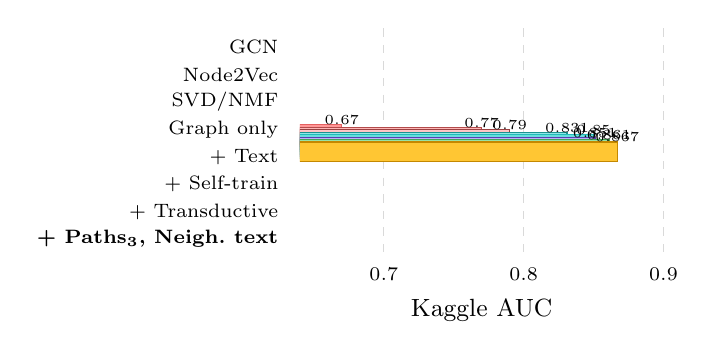
\begin{tikzpicture}
\begin{axis}[
    xbar,
    width=6.2cm, height=4.5cm,
    bar width=7pt,
    xlabel={\small Kaggle AUC},
    xmin=0.64, xmax=0.90,
    ytick={1,2,3,4,5,6,7,8},
    yticklabels={
        {\scriptsize GCN},
        {\scriptsize Node2Vec},
        {\scriptsize SVD/NMF},
        {\scriptsize Graph only},
        {\scriptsize + Text},
        {\scriptsize + Self-train},
        {\scriptsize + Transductive},
        {\scriptsize\bfseries + Paths\textsubscript{3}, Neigh.\ text}
    },
    y dir=reverse,
    ytick style={draw=none},
    xtick style={draw=none},
    tick label style={font=\scriptsize},
    axis line style={draw=none},
    xmajorgrids=true,
    grid style={dashed, gray!30},
    enlarge y limits=0.1,
    nodes near coords,
    nodes near coords style={font=\tiny\bfseries, /pgf/number format/fixed, /pgf/number format/precision=3},
    point meta=explicit,
]
\addplot[fill=coral!70, draw=coral!90!black] coordinates {(0.670,1) [0.670]};
\addplot[fill=coral!50, draw=coral!70!black] coordinates {(0.770,2) [0.770]};
\addplot[fill=coral!40, draw=coral!60!black] coordinates {(0.790,3) [0.790]};
\addplot[fill=skyblue!50, draw=skyblue!70!black] coordinates {(0.831,4) [0.831]};
\addplot[fill=skyblue!70, draw=skyblue!90!black] coordinates {(0.850,5) [0.850]};
\addplot[fill=violet!50, draw=violet!70!black] coordinates {(0.851,6) [0.851]};
\addplot[fill=mint!60, draw=mint!80!black] coordinates {(0.861,7) [0.861]};
\addplot[fill=gold!80, draw=darkgold] coordinates {(0.867,8) [0.867]};
\end{axis}
\end{tikzpicture}
\end{figure}

\begin{warningbox}
High-dimensional embeddings (SVD 128-d, Node2Vec, GCN) all \emph{decreased} AUC. With 10K training samples, the curse of dimensionality dominates. Scalar features win.
\end{warningbox}

%======================================================================
\section{Model Tuning \& Comparison}
%======================================================================

%----------------------------------------------------------------------
\subsection{Models}
%----------------------------------------------------------------------

\begin{center}
\small
\renewcommand{\arraystretch}{1.2}
\begin{tabular}{l c c}
\toprule
\textbf{Model} & \textbf{AUC} & \\
\midrule
\rowcolor{coral!10} GCN (2-layer) & 0.670 & \color{coral}\faIcon{times-circle} \\
Logistic Regression & 0.831 & \color{slate}\faIcon{minus-circle} \\
Random Forest & 0.845 & \color{slate}\faIcon{minus-circle} \\
CatBoost~\cite{prokhorenkova2018} & 0.861 & \color{mint!70!black}\faIcon{check-circle} \\
\rowcolor{gold!10} \textbf{HGB ensemble}~\cite{ke2017} & \textbf{0.867} & \color{darkgold}\faIcon{trophy} \\
\bottomrule
\end{tabular}
\end{center}

\textbf{HGB} (HistGradientBoosting): histogram-based gradient boosting inspired by LightGBM. Best single model thanks to efficient handling of our 36 features.

\textbf{CatBoost}: ordered boosting with built-in regularization. Similar Kaggle score but different error patterns — valuable for ensemble diversity.

\textbf{GCN}: 2-layer Graph Convolutional Network, end-to-end. Massively overfit on this small dataset, confirming deep learning is impractical here.

%----------------------------------------------------------------------
\subsection{Hyperparameter Tuning}
%----------------------------------------------------------------------

Grid search over 5 axes for HGB:

\begin{center}
\scriptsize
\renewcommand{\arraystretch}{1.15}
\begin{tabular}{>{\ttfamily\color{violet}}l l >{\bfseries\color{mint!70!black}}c}
\toprule
\normalfont\textbf{Parameter} & \textbf{Range} & \textbf{Best} \\
\midrule
learning\_rate & 0.02, 0.03, \textbf{0.05} & 0.05 \\
max\_depth & 2, \textbf{3}, 4 & 3 \\
max\_iter & 300, \textbf{400}, 500 & 400 \\
min\_samples\_leaf & 25, \textbf{40}, 50, 60 & 40 \\
l2\_regularization & \textbf{0.1}, 0.3, 0.5 & 0.1 \\
\bottomrule
\end{tabular}
\end{center}

CatBoost: \texttt{iter}=300, \texttt{lr}=0.05, \texttt{depth}=3, \texttt{l2}=10.

%----------------------------------------------------------------------
\subsection{Overfitting \& Mitigation}
%----------------------------------------------------------------------

Local OOF AUC (0.904) $\gg$ Kaggle (0.867). Two causes:
\begin{enumerate}
    \item \textbf{Graph feature leakage}: CV reuses the same adjacency. Positive validation edges remain in the graph, inflating CN/AA/RA. Honest CV (rebuilding graph per fold) gives OOF~$\approx$0.57.
    \item \textbf{Transductive leakage}: pair counts include test data, subtly biasing CV.
\end{enumerate}

\textbf{Mitigations}: 15-seed averaging, conservative regularization, single-round self-training at high threshold, and only trusting Kaggle scores for feature selection decisions.

%----------------------------------------------------------------------
\subsection{Ensemble}
%----------------------------------------------------------------------

Final: \textbf{HGB + CatBoost} (15 seeds each), combined via \textbf{rank averaging}. Since AUC is rank-based, converting predictions to ranks before blending eliminates calibration issues between models.

%======================================================================
\section{Conclusion}
%======================================================================

\begin{tcolorbox}[
  colback=mint!8, colframe=mint!70!black,
  arc=3pt, boxrule=0.6pt, left=4pt, right=4pt, top=3pt, bottom=3pt
]
\begin{enumerate}
    \item \textbf{Feature discipline}: 36 scalar features beat all high-dimensional approaches on this small dataset.
    \item \textbf{Transductive thinking}: exploiting test-set structure gave the single biggest boost (+0.011).
    \item \textbf{Leakage awareness}: analytically correcting paths$_3$ and neighborhood text features enabled genuine new signals without overfitting.
\end{enumerate}
\end{tcolorbox}

\vspace{4pt}
\small
\begin{thebibliography}{7}
\bibitem{liben2007} D.~Liben-Nowell, J.~Kleinberg. The link-prediction problem for social networks. \emph{JASIST}, 58(7), 2007.
\bibitem{adamic2003} L.~Adamic, E.~Adar. Friends and neighbors on the web. \emph{Social Networks}, 25(3), 2003.
\bibitem{katz1953} L.~Katz. A new status index derived from sociometric analysis. \emph{Psychometrika}, 18(1), 1953.
\bibitem{ke2017} G.~Ke et~al. LightGBM: A highly efficient gradient boosting decision tree. \emph{NeurIPS}, 2017.
\bibitem{prokhorenkova2018} L.~Prokhorenkova et~al. CatBoost: Unbiased boosting with categorical features. \emph{NeurIPS}, 2018.
\bibitem{zhou2004} D.~Zhou et~al. Learning with local and global consistency. \emph{NeurIPS}, 2004.
\bibitem{lu2011} L.~L{\"u}, T.~Zhou. Link prediction in complex networks: A survey. \emph{Physica A}, 390(6), 2011.
\end{thebibliography}

\end{document}
